\section{临近梯度下降法}

本节引入临近算子与临近梯度的概念,分析临近梯度下降法,并使用该方法求解具体的凸优化问题。

\subsection{凸优化模型}

考虑凸优化问题$\min\limits_{x\in \mathbb{R}^{n}} f(x) := g(x) + h(x)$,其中函数$g(x)$是可微的且Lipschitz连续,而$h(x)$则可能是连续但不处处可微的函数。
例如,在对优化的函数引入正则项时,就属于上述的凸优化模型,其中$h(x)=\|x\|_{1}$即$l_{1}$范数。对于这样的模型,可以采用临近梯度下降法求解最优解。

在应用临近梯度下降法进行优化时,通常对Lipschitz连续的部分即$g(x)$求梯度,但对于不处处可微的$h(x)$部分在无法求解梯度时,采用求临近梯度的方式代替。

\subsection{临近算子与临近梯度}

在对$h(x)$求临近梯度\cite{2014Prox}前,首先引入临近算子的概念,用于处理非光滑函数,计算求解一个距离$x$最近的点使得$h(x)$最小。

\begin{definition}\label{def_prox_1}
    对于一个凸函数$h(x)$,定义它的临近算子为

    \begin{equation}
        \mathop{\mathrm{prox_{h}}}(x) = \mathop{\mathrm{argmin}}\limits_{u\in \mathop{\mathrm{dom}} (h)}\{h(u)+\frac{1}{2}\|u-x\|^{2}\}.
    \end{equation}

\end{definition}

如果想进一步基于临近算子的概念定义临近梯度,并用于优化问题的求解,必须证明上述定义的临近算子唯一存在,这样对于一个给定的凸优化问题,其最优解才是唯一的。

\begin{theorem}\label{thm_prox_1}
    如果$h(x)$是一个定义在$\mathbb{R}^{n}$上的适当的闭凸函数,则对任意的$x\in \mathbb{R}^{n}$,$\mathop{\mathrm{prox_{h}}}(x)$的值唯一存在。
\end{theorem}

\begin{proof}
    假设$h(x)$至少在定义域内存在一点存在次梯度$\bm{g}$,由次梯度的定义可以得到

    \begin{equation}
        h(u)\geq h(v)+\langle \bm{g}, u-v\rangle, v\in \mathop{\mathrm{dom} (h)}.
    \end{equation}

    定义辅助函数

    \begin{equation}
        m(u)=h(u)+\frac{1}{2}\|u-x\|^{2}.
    \end{equation}

    可以得到
    \begin{equation}
        m(u)\geq h(v) + \langle \bm{g}, u-v\rangle + \frac{1}{2}\|u-x\|^{2}.
    \end{equation}

    因此,$m(u)$是适当闭函数,由Weierstrass定理可知其存在最小值。

    同时,注意到$m(u)$是强凸函数,由强凸函数的性质可知,$m(u)$最小值唯一。

    综上所述,$\mathop{\mathrm{prox_{h}}}(x)$的值存在且唯一。
\end{proof}

以$l_{1}$范数为例给出其临近算子的计算,这常被用于作为优化问题的$l_{1}$正则项,例如在Lasso问题中也将运用$l_{1}$范数的临近算子计算。

\begin{problem}\label{exp_prox_1}
    求解$l_{1}$范数的临近算子,即求

    \begin{equation}
        \mathop{\mathrm{prox_{h}}}(x), h(x)=t\|x\|_{1}, t > 0.
    \end{equation}
\end{problem}

\begin{solution}
    给定$l_{1}$范数$h(x)=t\|x\|_{1}, t>0$,按照定义\ref{def_prox_1}可以得到其临近算子的形式为

    \begin{equation}
        \mathop{\mathrm{prox_{h}}}(x) = \mathop{\mathrm{argmin}}\limits_{u\in \mathbb{R}^{n}}
        \begin{cases}
            tu + \frac{1}{2}(u-x)^{2}, u>0      ,\\
            -tu + \frac{1}{2}(u-x)^{2}, u\leq 0 .\\
        \end{cases}
    \end{equation}

    进一步考虑,当$x>t$时,$\mathop{\mathrm{prox_{h}}}(x) = x-t$;
    当$x<-t$时,$\mathop{\mathrm{prox_{h}}}(x) = x+t$;
    当$-t\leq x\leq t$时,$\mathop{\mathrm{prox_{h}}}(x) = 0$,即$h(x)$唯一不可微的点。

    综上所述,可以引入符号函数简化上述分类,即
    
    \begin{equation}\label{eq_prox_3}
        \mathop{\mathrm{prox_{h}}}(x) = \mathop{\mathrm{sgn}}(x)\max\{|x|-t, 0\}.
    \end{equation}
    
    其中,$\mathop{\mathrm{sgn}}(x)$的定义与函数图像如下。
    \begin{definition}
        对于$\mathop{\mathrm{sgn}}(x)$,定义
        \begin{equation}
            \mathop{\mathrm{sgn}}(x) = 
            \begin{cases}
                1, &x > 0, \\
                0, &x = 0, \\
                -1, &x < 0.
            \end{cases}
        \end{equation}
    \end{definition}

    $\mathop{\mathrm{sgn}}(x)$函数的图像如下图\ref{figure_sgn}所示。
    \begin{figure}[hbtp]
        \centering
        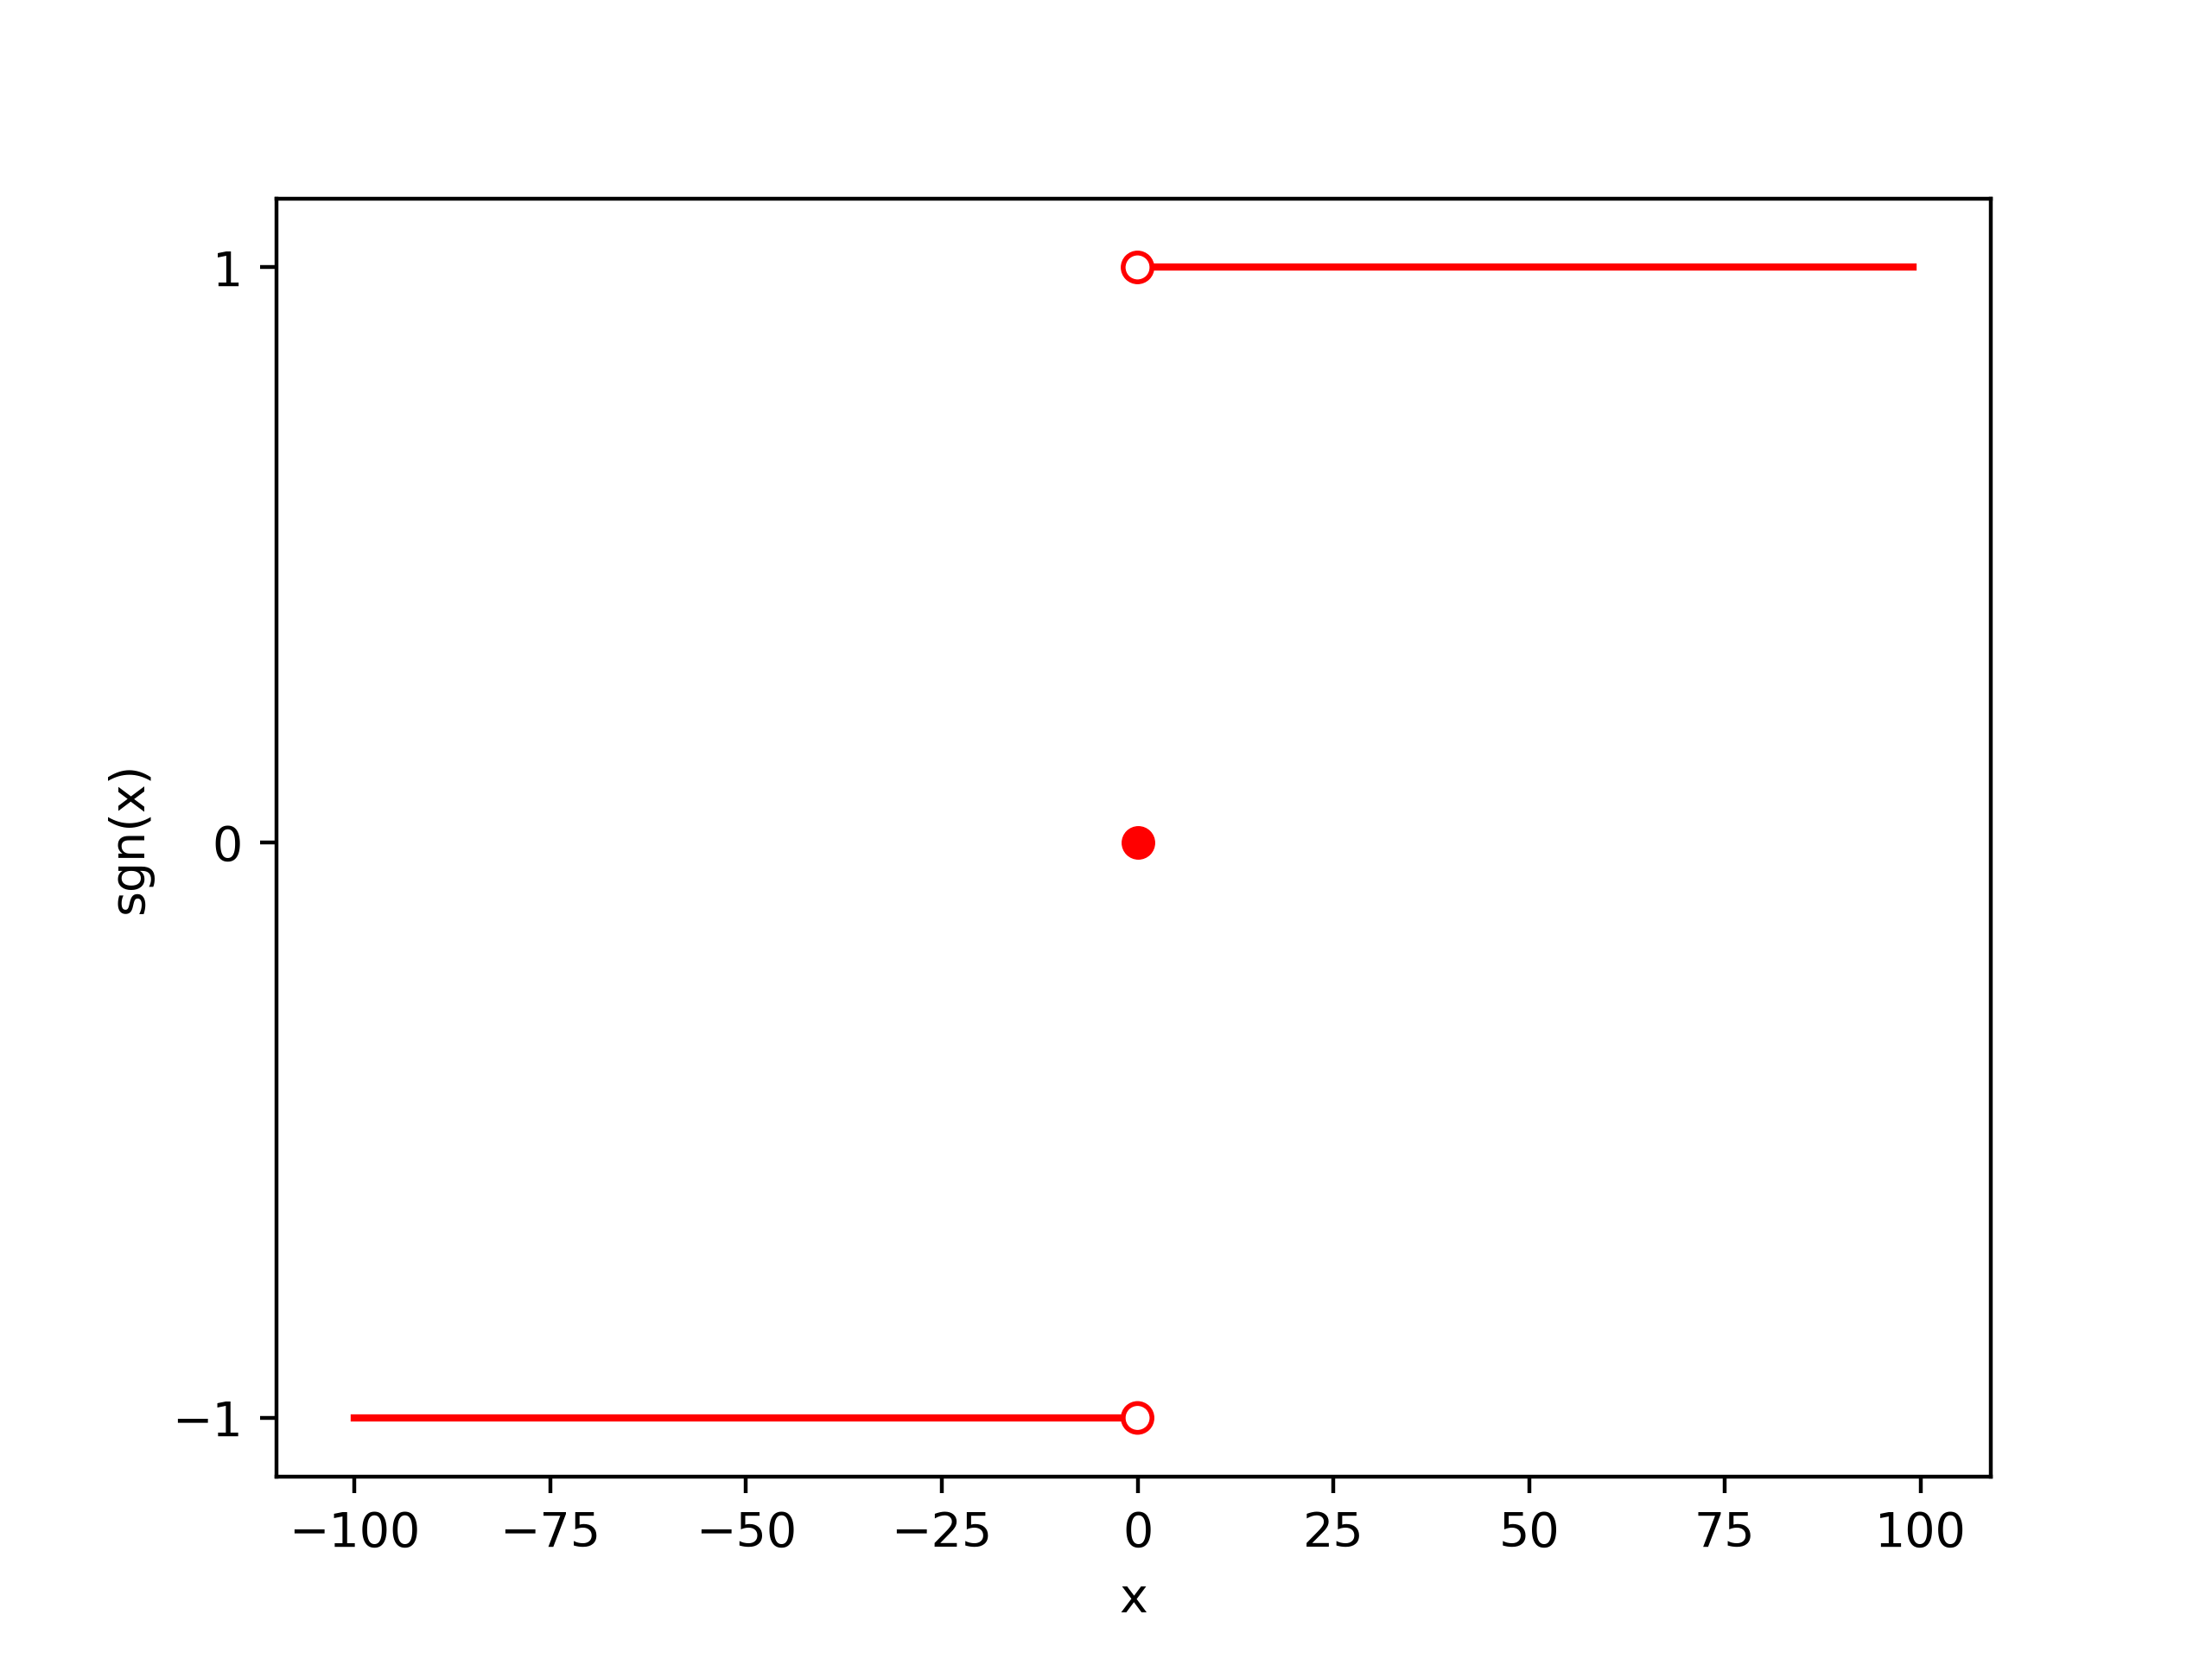
\includegraphics[width=100mm]{./Figures/sgn_figure.png}
        \caption{$\mathop{\mathrm{sgn}}(x)$函数图像}
        \label{figure_sgn}
    \end{figure}
\end{solution}

由定理\ref{thm_prox_1}可进一步定义临近梯度的概念,用于作为梯度的扩展概念,处理一个可分解的函数中非光滑的部分,而对于光滑的部分则使用梯度计算。

\begin{definition}\label{def_prox_2}
    对于$f(x) := g(x)+h(x)$,其中$g(x)$是连续可微的且Lipschitz连续,$h(x)$是连续但不处处可微的,定义它的临近梯度为

    \begin{equation}
        \tilde{\nabla} f(x) = x - \mathop{\mathrm{prox_{\alpha h}}}(x-\alpha \nabla g(x)),
    \end{equation}

    其中,$\alpha > 0$,在临近梯度下降法中的意义同梯度下降法中的步长。
\end{definition}

显然,当非光滑的部分$h(x)=0$时,临近梯度$\tilde{\nabla} f(x)=\alpha \nabla g(x)=\alpha \nabla f(x)$即梯度。这表明了临近梯度的定义是梯度的扩展,也说明了梯度是临近梯度的特殊情况。

\subsection{临近梯度下降法}

对于凸优化问题$\min\limits_{x\in \mathbb{R}^{n}} f(x) := g(x) + h(x)$,其中,$g(x)$是可微且Lipschitz连续的函数,而$h(x)$则是不处处可微的凸函数。

针对光滑的部分$g(x)$采用计算梯度的方式,而对于非光滑的部分$h(x)$采用计算临近算子的方式,下面给出迭代公式

\begin{equation}
    \begin{cases}
        y^{k+1} = x^{k} - \alpha_{k}\nabla g(x^{k}) ;\\
        x^{k+1} = \mathop{\mathrm{prox_{\alpha_{k} h}}}(y^{k+1}).
    \end{cases}
\end{equation}

或者将两次迭代合并写成

\begin{equation}\label{eq_prox_2}
    x^{k+1} = \mathop{\mathrm{prox_{\alpha_{k} h}}}(x^{k} - \alpha_{k}\nabla g(x^{k})),
\end{equation}

其中,$\alpha_{k}$表示第$k$次迭代时算法选取的步长,通常$0<\alpha<1$;$x^{k}$表示第$k$次的迭代。

由定义\ref{def_prox_2}对临近梯度的定义可知,临近梯度下降法其实是计算了使得$\tilde{\nabla} f(x)=0$的解,并将其作为问题的最优解。

结合迭代公式\ref{eq_prox_2}与初始化设置,可以将临近梯度下降法总结为如下算法。

\begin{algorithm}\label{alg_prox_1}
    \SetKwInOut{Input}{输入}\SetKwInOut{Output}{输出}

    \SetAlgoLined
    \Input{$f(x):=g(x)+h(x)$,初始化设置$k=0$}
    \Output{最优解$x^{*}$}

    \While{未收敛} {
        $x^{k+1} = \mathop{\mathrm{prox_{\alpha_{k} h}}}(x^{k} - \alpha_{k}\nabla g(x^{k}))$

        $k \leftarrow k+1$
    }
    \caption{临近梯度下降法}
\end{algorithm}

\subsection{算法分析}

首先,对于问题\ref{eq_prox_1},临近梯度下降法实际是对非光滑部分$g(x)$在$x^{k}$处的Taylor展开再加上二次项,同时保留非光滑部分$h(x)$,对该展开式求极小来作为每次迭代的近似。

\begin{equation}
    \begin{split}
        x^{k+1} &=  \mathop{\mathrm{argmin}}\limits_{u\in \mathop{\mathrm{dom}} (h)}\{\alpha_{k}h(u) + \frac{1}{2}\|u-(x^{k}-\alpha_{k}\nabla g(x^{k}))\|^{2}\} \\
                &= \mathop{\mathrm{argmin}}\limits_{u\in \mathop{\mathrm{dom}} (h)} \{h(u)+g(x^{k})+\langle \nabla g(x^{k}), u-x^{k} \rangle + \frac{1}{2\alpha_{k}}\|u-x^{k}\|^{2}\}.
    \end{split}
\end{equation}

其次,临近梯度下降法对光滑的部分做显式的梯度下降,对非光滑部分根据其性质与结构使用临近算子做隐式的梯度下降进行求解。这相比一般的梯度下降法能够求解更多的问题,也是临近梯度下降法的优势。

最后,考虑算法\ref{alg_prox_1}的收敛性分析。

\begin{theorem}
    假设给定步长为常数,即$\alpha_{k}=\alpha\in (0, \frac{1}{L}]$,后记作$\alpha$,其中$L$表示Lipschitz连续的部分$g(x)$满足$\|\nabla g(x)-\nabla g(y)\| \leq L\|x-y\|, \forall x, y \in \mathbb{R}^{n}$,迭代点$x^{k}$处的函数值$f(x^{k})$以$O(\frac{1}{k})$的速率收敛到最优解$x^{*}$
\end{theorem}

\begin{proof}
    由下降引理可得

    \begin{equation*}
        g(y) \leq g(x) + \langle \nabla g(x), y-x \rangle + \frac{L}{2}\|x-y\|^{2}, \forall x, y \in \mathbb{R}^{n}.
    \end{equation*}

    令$y=x-\alpha\tilde{\nabla} g(x)$,有

    \begin{equation*}
        g(x-\alpha\tilde{\nabla} g(x)) \leq g(x) - \alpha \langle \nabla g(x), y-x \rangle \tilde{\nabla} g(x) + \frac{\alpha^{2}L}{2}\|\tilde{\nabla} g(x)\|^{2}.
    \end{equation*}

    由$0<t\leq \frac{1}{L}$可知,

    \begin{equation*}
        g(x-\alpha\tilde{\nabla} g(x)) \leq g(x) - \alpha \langle \nabla g(x), y-x \rangle \tilde{\nabla} g(x) + \frac{\alpha}{2}\|\tilde{\nabla} g(x)\|^{2}.
    \end{equation*}

    由$g(x), h(x)$为凸函数,对$\forall z \in \mathop{\mathrm{dom}} (f)$,有
    \begin{equation*}
        g(x) \leq g(z) - \langle \nabla g(x), z-x  \rangle.
    \end{equation*}

    整理可得,对$\forall z \in \mathop{\mathrm{dom}} (f)$,有
    \begin{equation*}
        f(x-\alpha\tilde{\nabla} g(x)) \leq f(z) + \langle \tilde{\nabla}g(x), z-x \rangle - \frac{\alpha}{2}\|\tilde{\nabla} g(x)\|^{2}.
    \end{equation*}

    记第$k+1$次迭代为$x^{k+1}=x^{k}-\alpha\tilde{\nabla}g(x^{k})$,
    
    令$z=x^{*}$为问题的最优解,有

    \begin{equation}
        \begin{split}
            f(x^{k+1})-f(x^{*}) &\leq \langle \tilde{\nabla}g(x^{k}), x^{k}-x^{*} \rangle - \frac{\alpha}{2}\|\tilde{\nabla}g(x^{k})\|^{2} \\
            &=\frac{1}{2\alpha}(\|x^{k}-x^{*}\|^{2} - \|x^{k}-x^{*}-\alpha\tilde{\nabla}g(x^{k})\|^{2}) \\
            &=\frac{1}{2\alpha}(\|x^{k}-x^{*}\|^{2} - \|x^{k+1}-x^{*}\|^{2}).
        \end{split}
    \end{equation}

    将前$k$次迭代的结果累加代入上式可得,
    \begin{equation}
        \begin{split}
            \sum_{i=1}^{k}(f(x^{i} - f(x^{*}))) &\leq \frac{1}{2\alpha}\sum_{i=1}^{k}(\|x^{i-1}-x^{*}\|^{2} - \|x^{i}-x^{*}\|^{2}) \\
            &= \frac{1}{2\alpha}(\|x^{0}-x^{*}\|^{2} - \|x^{k}-x^{*}\|^{2}) \\
            &\leq \frac{1}{2\alpha} \|x^{0} - x^{*}\|^{2}.
        \end{split}
    \end{equation}

    其中,$x^{0}$同算法\ref{alg_prox_1}中的初始化设置。

    因此,
    \begin{equation}
        f(x^{k}-f(x^{*})) \leq \frac{1}{2k\alpha}\|x^{0}-x^{*}\|^{2}.
    \end{equation}

    综上所述,迭代点$x^{k}$处的函数值$f(x^{k})$以$O(\frac{1}{k})$的速率收敛到最优解$x^{*}$。
\end{proof}

\subsection{应用}

以Lasso问题为例,使用临近梯度下降法求解该优化问题。

\begin{problem}
    求解Lasso问题,即求
    \begin{equation}
        \mathop{\mathrm{min}\limits_{x}} f(x) := \frac{1}{2}\|\bm{A} \bm{x}-\bm{b}\|_{2}^{2} + \mu\|\bm{x}\|_{1}.
    \end{equation}
\end{problem}

\begin{solution}
    考虑凸函数$f(\bm{x})$可以分解为光滑的部分$g(\bm{x})=\frac{1}{2}\|\bm{A} \bm{x}-\bm{b}\|_{2}^{2}$,与非光滑的部分$h(\bm{x})=\mu\|\bm{x}\|_{1}$,

    对光滑部分求梯度可以得到

    \begin{equation*}
        \nabla g(\bm{x}) = \bm{A}^{T}(\bm{A} \bm{x}-\bm{b}).
    \end{equation*}

    由\ref{eq_prox_3},对非光滑部分求临近算子可以得到

    \begin{equation*}
        \mathop{\mathrm{prox_{\alpha_{k}h}}}(\bm{x}) = \mathop{\mathrm{sgn}}(\bm{x})\max\{|\bm{x}|-\alpha_{k}\mu, 0\},
    \end{equation*}

    其中,$\alpha_{k}$表示第$k$次迭代的步长。

    由迭代公式\ref{eq_prox_2},可以得到

    \begin{equation}
        \begin{split}
            \bm{x}^{k+1} &= \mathop{\mathrm{prox_{\alpha_{k}h}}}(\bm{x}^{k} - \alpha_{k}\nabla g(\bm{x}^{k})) \\
            &=\mathop{\mathrm{prox_{\alpha_{k}h}}}(\bm{x}^{k} - \alpha_{k}\bm{A}^{T}(\bm{A} \bm{x}^{k}-\bm{b})) \\
            &=\mathop{\mathrm{sgn}}(\bm{x}^{k} - \alpha_{k}\bm{A}^{T}(\bm{A} \bm{x}^{k}-\bm{b}))\max\{\|\bm{x}^{k} - \alpha_{k}\bm{A}^{T}(\bm{A} \bm{x}^{k}-\bm{b})\|-\alpha_{k}\mu, 0\}
        \end{split}
    \end{equation}

    使用Python对该问题求解,可以得到结果如图\ref{figure_prox}所示,代码在附录中给出。其中,alpha表示算法\ref{alg_prox_1}中的学习率。可以看出,随着学习率的增加,算法收敛的速度也越快,特别地,在学习率较小的时候,算法未能在给定的300个epoch内收敛。

    \begin{figure}[hbtp]
        \centering
        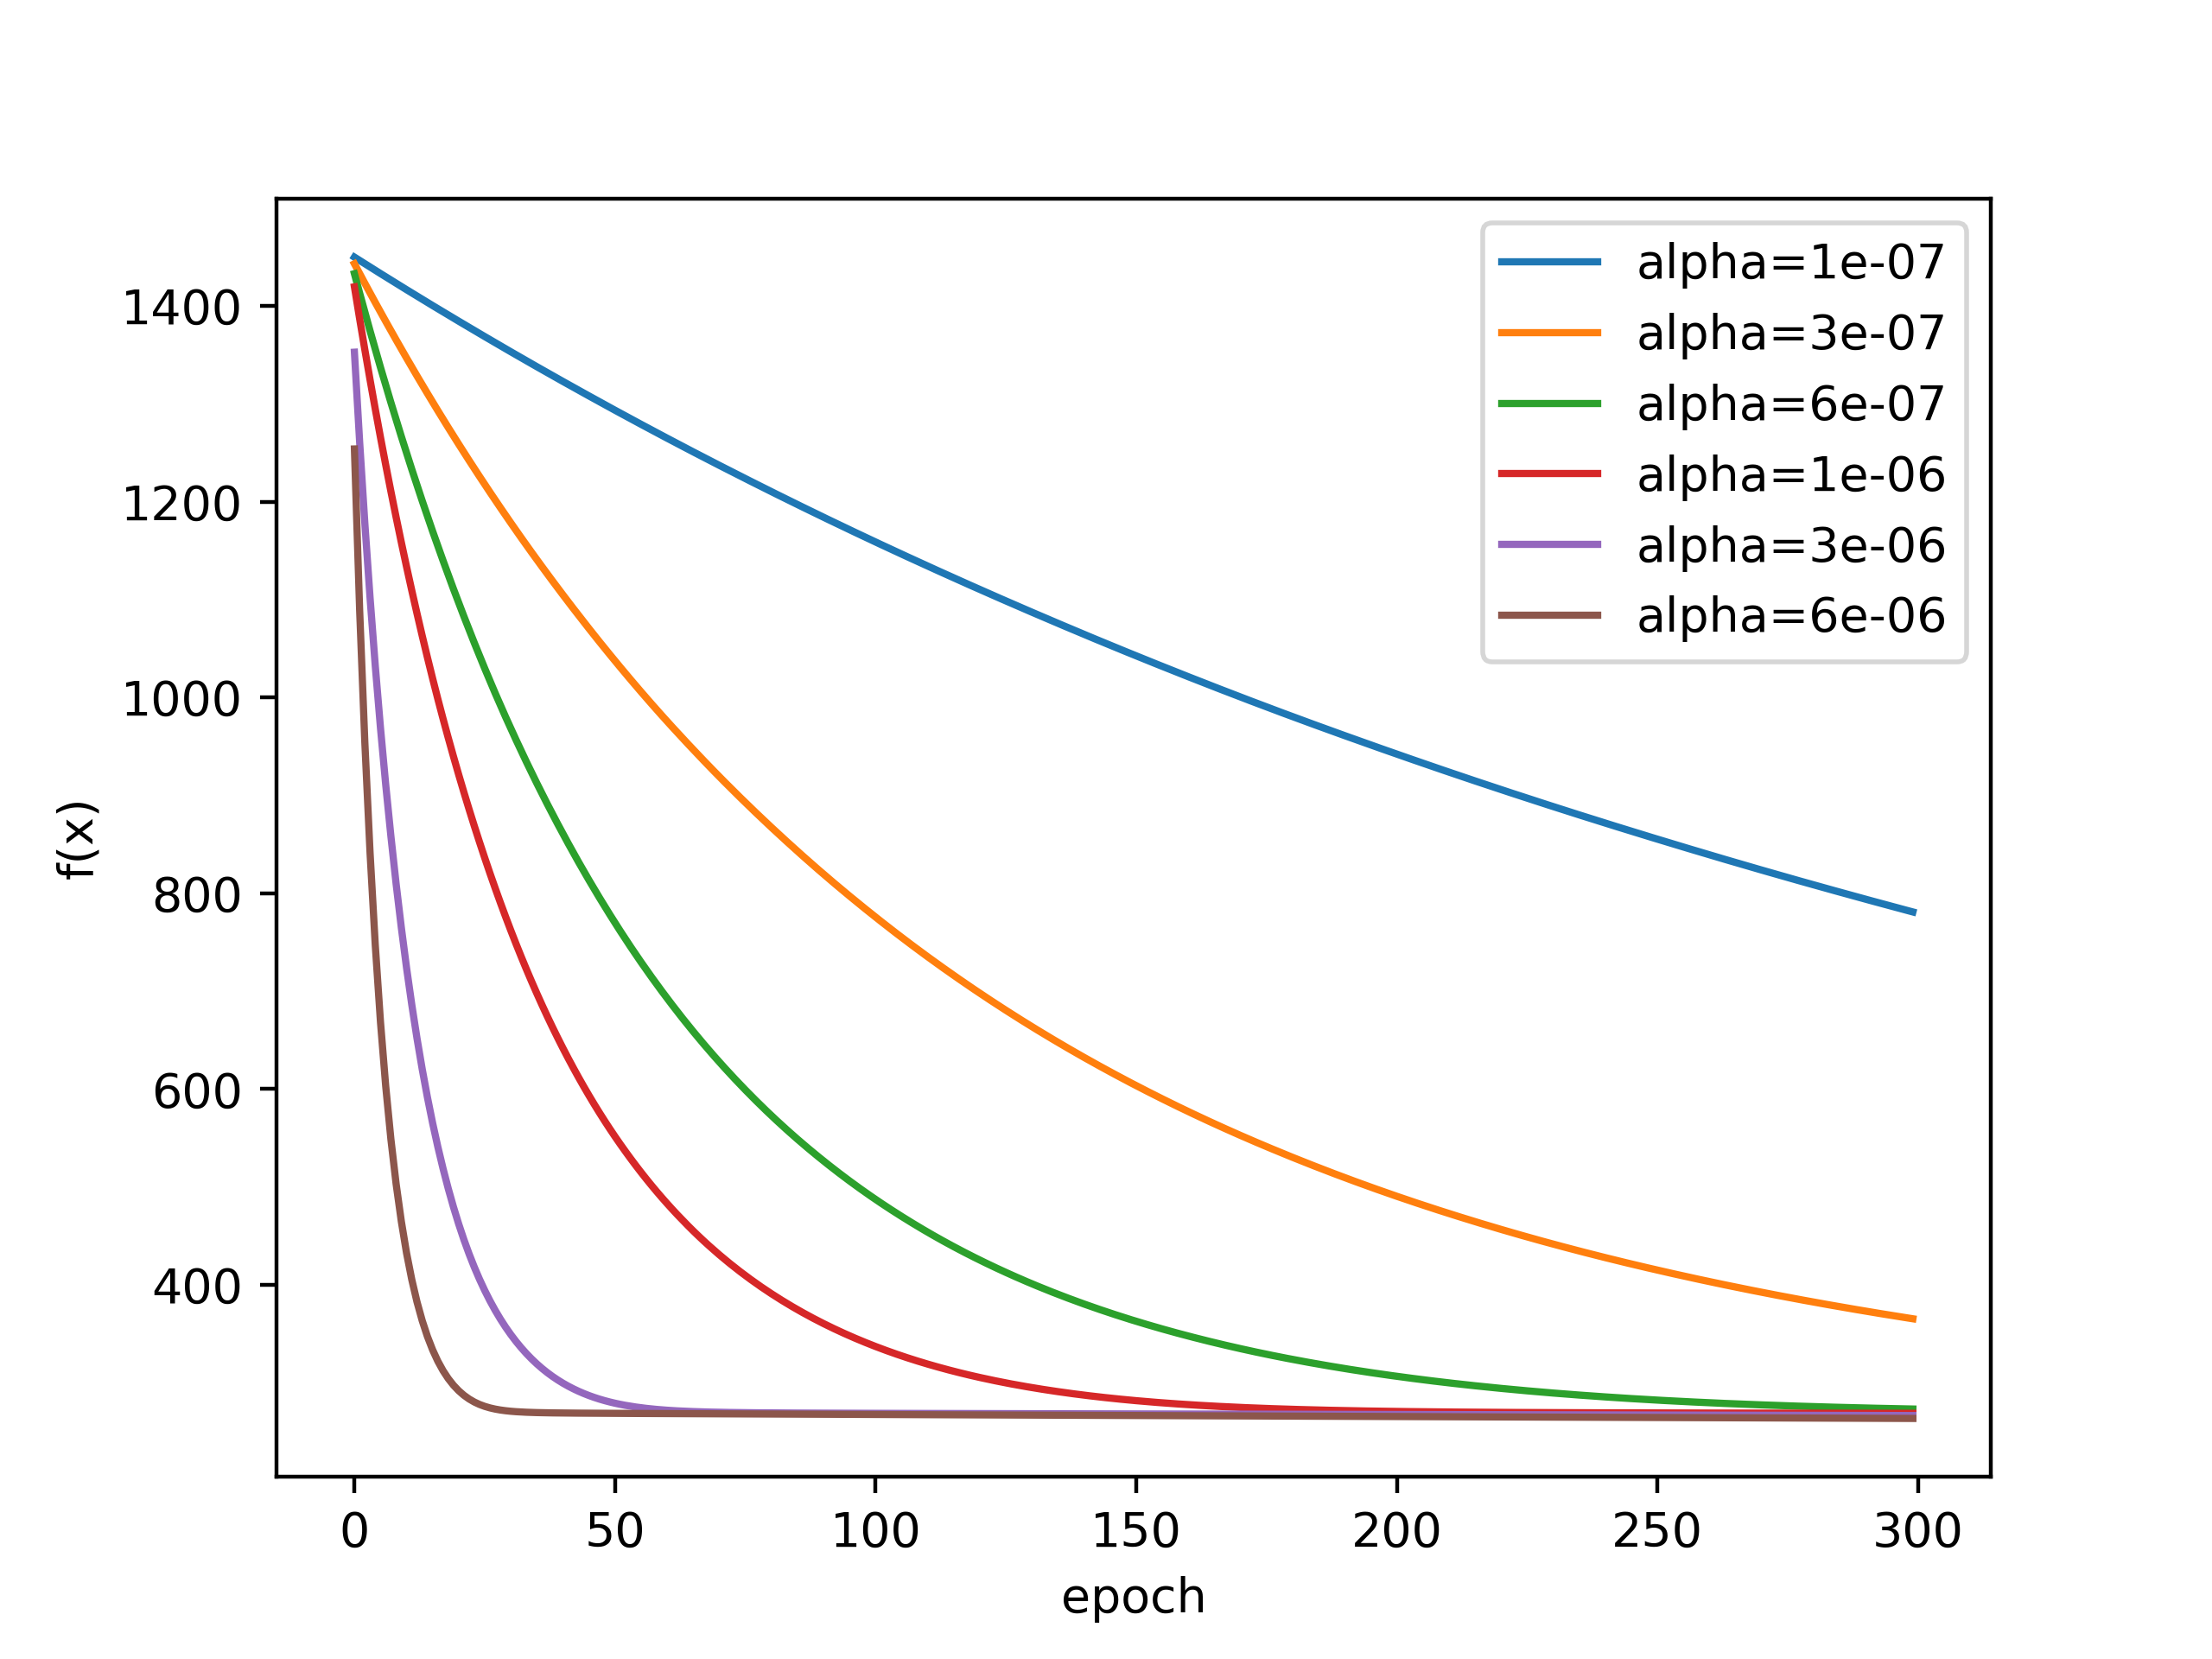
\includegraphics[width=150mm]{./Figures/prox.png}
        \caption{Python实现临近梯度下降法求解Lasso问题}
        \label{figure_prox}
    \end{figure}
\end{solution}